% Start of Apache Spark section

% \subsection*{Giao cho: Tuấn Kiệt Trần}
% \subsection*{Trạng thái: Hoàn thành}
$\indent$Apache Spark là một hệ thống động lực phân tích thống nhất cho xử lý dữ liệu quy mô lớn. Đặc điểm chính của Apache Spark là \textit{in-memory cluster computing}, tăng tốc độ xử lý của ứng dụng. Spark cung cấp giao diện lập trình cho việc lập trình toàn bộ cụm máy với \textit{tính song song dữ liệu và khả năng chịu lỗi} ngầm. Nó được thiết kế để xử lý nhiều loại công việc như ứng dụng batch, thuật toán lặp, truy vấn tương tác và xử lý dữ liệu liên tục.

\subsection{Hệ sinh thái Spark}

\subsubsection*{\textbf{Spark Core}}

Spark Core là động cơ cơ bản cho xử lý dữ liệu lớn phân tán và song song. Thêm vào đó, các thư viện bổ sung được xây dựng trên cơ bản cho phép các công việc đa dạng như xử lý luồng, SQL và học máy. Nó chịu trách nhiệm quản lý bộ nhớ và khôi phục lỗi, lập lịch, phân phối và giám sát công việc trên một cụm và tương tác với hệ thống lưu trữ.

\subsubsection*{\textbf{Spark Streaming}}

Spark Streaming là thành phần của Spark được sử dụng để xử lý dữ liệu luồng thời gian thực. Spark Streaming cho phép xử lý dữ liệu luồng có khả năng mở rộng, xử lý lưu lượng cao và chống lỗi của dữ liệu luồng trực tiếp. Dữ liệu có thể được nhập từ nhiều nguồn như Kafka, Kinesis hoặc ổ cắm TCP và có thể được xử lý bằng các thuật toán phức tạp được biểu diễn bằng các hàm cấp cao như \texttt{map}, \texttt{reduce}, \texttt{join} và \texttt{window}. Cuối cùng, dữ liệu được xử lý có thể được đẩy ra hệ thống tệp, cơ sở dữ liệu và bảng điều khiển thời gian thực.

\begin{figure}[H]
    \centering
    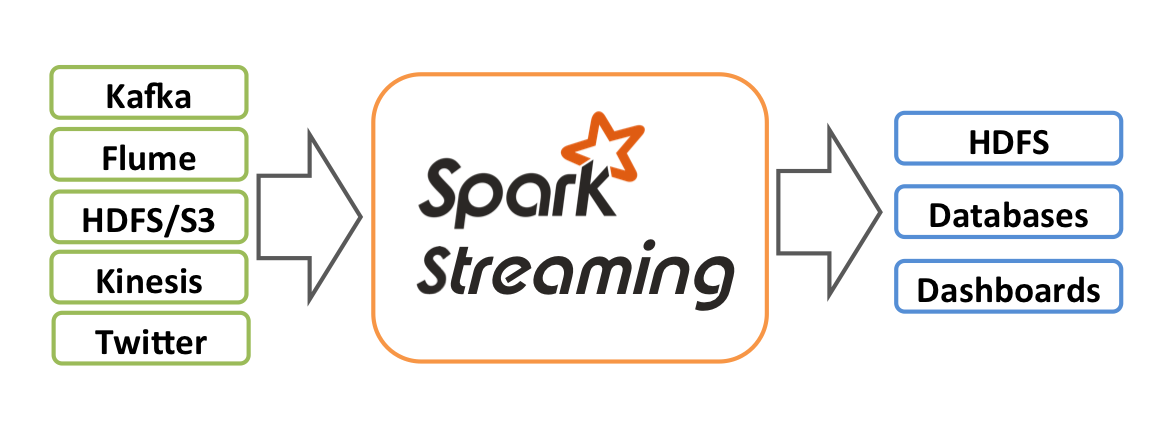
\includegraphics[width=0.8\linewidth]{Images/3.2-spark-eco.png}
    \vspace{1em}
    \caption{Hệ sinh thái Spark}
    \label{fig:eco}
\end{figure}

Spark Streaming cung cấp một trừu tượng cấp cao gọi là \textit{discretized stream} hoặc \textit{DStream}, đại diện cho một luồng liên tục của dữ liệu. DStream có thể được tạo ra từ dữ liệu đầu vào từ nguồn như Kafka, và Kinesis hoặc bằng cách áp dụng các hoạt động cấp cao trên các DStream khác. Nội tại, một DStream được biểu diễn như một chuỗi các \texttt{RDDs}.

\begin{figure}[H]
    \centering
    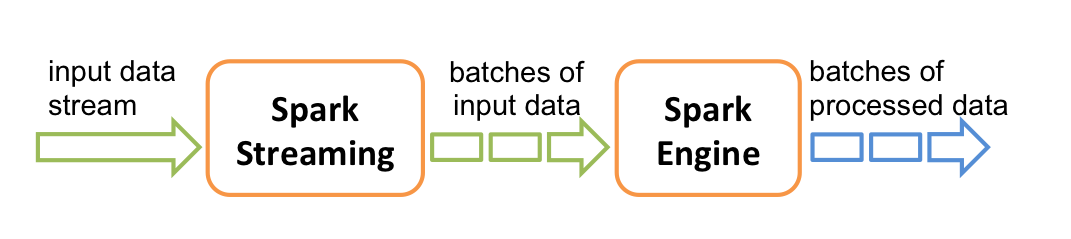
\includegraphics[width=1\linewidth]{Images/3.2-spark-flow.png}
    \vspace{1em}
    \caption{Luồng xử lý dữ liệu}
    \label{fig:flow}
\end{figure}

\subsubsection*{\textbf{GraphX}}

GraphX là API của Spark cho đồ thị và tính toán đồ thị song song. Do đó, nó mở rộng trừu tượng RDD của Spark với một Đồ thị Phân tán Bền vững. Ở mức cao, GraphX mở rộng trừu tượng RDD của Spark bằng cách giới thiệu Đồ thị Phân tán Bền vững (một đồ thị hướng nhiều cạnh với thuộc tính đính kèm cho mỗi đỉnh và cạnh).

\subsubsection*{\textbf{MLlib (Học máy)}}

MLlib viết tắt của Machine Learning Library. Spark MLlib được sử dụng để thực hiện học máy trong Apache Spark.

Ở mức cao, nó cung cấp các công cụ như:

\begin{itemize}
    \item Thuật toán ML: các thuật toán học thông thường như phân loại, hồi quy, phân cụm và lọc cộng tác
    \item Tạo đặc điểm: trích xuất đặc điểm, chuyển đổi, giảm chiều và lựa chọn
    \item Đường ống: công cụ xây dựng, đánh giá và điều chỉnh ống ML
    \item Bền vững: lưu và tải thuật toán, mô hình và ống
    \item Tiện ích: đại số tuyến tính, thống kê, xử lý dữ liệu, v.v.
\end{itemize}

\subsection{Kiến trúc Spark}

Apache Spark có một kiến trúc lớp chặt chẽ được định nghĩa rõ ràng, trong đó tất cả các thành phần và lớp Spark đều được liên kết lỏng lẻo. Kiến trúc này được tích hợp với các phần mở rộng và thư viện đa dạng. Kiến trúc Apache Spark dựa trên hai trừu tượng chính:

\begin{itemize}
    \item \textit{Resilient Distributed Dataset (RDD)}
    \item \textit{Directed Acyclic Graph (DAG)}
\end{itemize}

\subsubsection*{\textbf{Resilient Distributed Dataset (RDD)}}

RDD là cơ sở của bất kỳ ứng dụng Spark nào. RDD viết tắt của:

\begin{itemize}
    \item \textit{Resilient:} Chống lỗi và có khả năng xây dựng lại dữ liệu khi xảy ra lỗi
    \item \textit{Distributed:} Phân phối dữ liệu giữa nhiều nút trong một cụm
    \item \textit{Dataset:} Tập hợp dữ liệu được phân vùng với các giá trị
\end{itemize}

Ở mức cao, mỗi ứng dụng Spark bao gồm một \textit{chương trình trình điều khiển} chạy hàm \texttt{main} của người dùng và thực hiện nhiều \textit{hoạt động song song} trên một cụm. RDD được tạo ra bằng cách bắt đầu với một tệp trong hệ thống tệp Hadoop (hoặc bất kỳ hệ thống tệp Hadoop nào khác được hỗ trợ), hoặc một bộ sưu tập Scala hiện tại trong chương trình điều khiển, và biến đổi nó. Người dùng cũng có thể yêu cầu Spark \textit{lưu giữ} một RDD trong bộ nhớ, cho phép nó được sử dụng lại hiệu quả trong các hoạt động song song. Cuối cùng, RDD tự động phục hồi từ sự cố nút.

\subsubsection*{\textbf{Directed Acyclic Graph (DAG)}}

DAG là một đồ thị hướng có hạn không có chu kỳ. Số \textit{đỉnh} và \textit{cạnh} có giá trị hữu hạn, mỗi cạnh được hướng từ một đỉnh này sang một đỉnh khác. Nó chứa một chuỗi các đỉnh sao cho mỗi cạnh được hướng từ trước đến sau trong chuỗi. Nó là một tổng quát nghiêm túc của mô hình \textbf{MapReduce}. Các hoạt động DAG có thể thực hiện tối ưu toàn cầu hơn so với các hệ thống khác như MapReduce.
\\

DAG của Apache Spark cho phép người dùng nghiên cứu chi tiết từng bước trong một giai đoạn. Trong \textit{góc nhìn giai đoạn,} chi tiết của tất cả các \textbf{RDDs} thuộc giai đoạn đó được mở rộng. Bộ lập lịch chia RDD Spark thành các \textit{giai đoạn} dựa trên các biến đổi khác nhau được áp dụng.
\newpage
\subsection{Tính toán Phân tán}

Để đạt được tính toán phân tán, cần phải quản lý tài nguyên và công việc trên một cụm máy. Quản lý tài nguyên liên quan đến việc đảm bảo trạng thái máy có sẵn cho công việc hiện tại, trong khi quản lý công việc liên quan đến việc phối hợp mã và dữ liệu trên cụm.

Một ứng dụng Spark bao gồm một chương trình trình điều khiển và thực hiện tính toán song song trên một cụm. Để bắt đầu một ứng dụng Spark, chương trình trình điều khiển chạy trên máy chủ sẽ đầu tiên khởi tạo một đối tượng SparkContext. Đối tượng SparkContext này sẽ giao tiếp với một quản lý cụm, có thể là quản lý cụm tự đứng của Spark, Mesos, YARN hoặc Kubernetes, để có được tài nguyên cho ứng dụng này. Sau đó, đối tượng SparkContext sẽ gửi mã ứng dụng và các nhiệm vụ đến các nút làm việc.

Đối với một ứng dụng, một nút làm việc có thể có nhiều thực thi, tùy thuộc vào số lượng CPU có sẵn trên nút làm việc này. Trong quá trình tính toán cho một ứng dụng, mỗi thực thi giữ dữ liệu trong bộ nhớ hoặc lưu trữ đĩa và thực hiện các nhiệm vụ. Như vậy, các thực thi được cô lập với nhau và các nhiệm vụ cho cùng một ứng dụng chạy song song.

\begin{figure}[H]
    \centering
    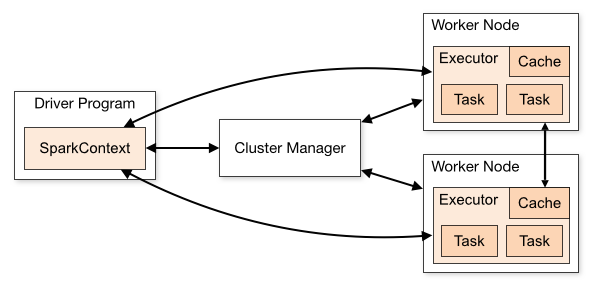
\includegraphics[width=0.7\linewidth]{Images/3.2-dist.png}
    \vspace{1em}
    \caption{Một mô hình tính toán phân tán sử dụng Spark}
    \label{fig:distributed}
\end{figure}

\subsection{Đánh giá công nghệ}
Apache Spark là một công cụ ETL rất mạnh mẽ. Nhiều giải pháp dữ liệu hiện đại sử dụng nó làm trọng tâm để thực hiện các nhiệm vụ kỹ thuật và phân tích phức tạp.

Tuy nhiên, không mọi công việc đều dễ dàng tích hợp với Spark. Hãy xem xét tình hình radar hiện tại của chúng tôi như một ví dụ. Để thực hiện việc chuyển đổi định dạng tệp, dường như chỉ có một loại công cụ hỗ trợ nhiệm vụ này: LROSE từ NCAR \cite{lrose}. Ngoài NCAR, Hầu như không có trang web hoặc trang nào cung cấp chi tiết về cách phân tích loại tệp này.

Do sự hiếm có của công việc này, chúng tôi buộc phải sử dụng bất kỳ giải pháp nào đã có, mà không có sự lựa chọn nào khác.

Spark có thể thực hiện tốt với nhiều công nghệ và cơ sở hạ tầng hiện có. Tệp CSV, cơ sở dữ liệu SQL và tài nguyên mạng thường được sử dụng phổ biến với công cụ phân tích này. Việc viết một plugin có thể là một giải pháp, tuy nhiên, sự khó khăn khi học cách phát triển một tiện ích mở rộng có thể là một thách thức lớn và cũng làm chậm quá trình phát triển.

Chính vì lý do này, chúng tôi đã chọn Apache Airflow làm trung tâm điều phối. Thực tế, việc xây dựng một giải pháp máy tính đồng nghĩa với việc học mọi thứ liên quan đến lập trình. Tuy nhiên, hệ sinh thái của Airflow cung cấp nhiều tiện ích mở rộng đã được xây dựng sẵn, giúp tương tác một cách dễ dàng với các hệ thống ngoại vi. Điều này, về thực tế, sẽ làm cho hệ thống trở nên linh hoạt hơn khi làm việc với bất kỳ giải pháp cụ thể nào.